% intro.tex
% Section 1: Introduction

\section{Introduction}
\label{sec:intro}

Game theory first asks whether a solution exists. \Citet{Neumann1928} showed that every
finite two-person zero-sum game has a value together with a pair of optimal
mixed strategies, and \citet{vNM1944} incorporated
this result into a general theory of economic behavior. \citet{Nash1951}
extended equilibrium existence to finite games with any finite number of players
and general payoff interactions, well beyond strictly
competitive play.

Mechanism design asks how the rules of interaction should be chosen. In
the standard quasilinear setting, the Vickrey--Clarke--Groves family showed how
to make truthful reporting a dominant strategy by charging each participant for
the externality it imposes~\citep{Vickrey1961,Clarke1971,Groves1973}, and
\citet{Myerson1981} characterized the
revenue-maximizing auction for the single-item Bayesian
setting. Impossibility results identify combinations of
domain restrictions and desiderata that cannot be satisfied
simultaneously~\citep{Arrow1951,Gibbard1973,Satterthwaite1975}.
Together, such results frame mechanism design as the selection of rules under
explicit incentive and feasibility constraints.

Once a solution concept has been defined and its existence established, the
next question is how to compute a solution. Algorithmic game theory studies
this question for different game representations and solution concepts
~\mbox{\citep{NisanRoughgardenTardosVazirani2007}}. Computing a Nash
equilibrium is PPAD-complete in general, and remains so with only two
players~\citep{DaskalakisGoldbergPapadimitriou2009,ChenDengTeng2009}. Even
classical constructive procedures can follow exponentially long
paths~\citep{LemkeHowson1964,SavaniVonStengel2006}. Established approaches weaken
the solution concept or exploit a restricted game's structure, often while
accepting approximation.

\subsection{How Learning Changes Computation}
\label{sec:intro:change}

Learning can amortize computation across related instances. An amortized method
trains a conditional rule on a family of related cases and reuses that rule on
new cases. This is the standard setup in amortized optimization and
inference~\citep{Amos2022Amortized,KingmaWelling2014}, and it has also been used
in strategic systems. In heads-up no-limit poker, learned counterfactual values
and continual re-solving are among the methods that have produced expert-level
play~\citep{Moravcik2017,BrownSandholm2018,BrownReBeL2020}. Self-play with
learned policy and value networks mastered board games from their rules, and
league training produced a StarCraft II agent at grandmaster
level~\citep{Silver2018,Vinyals2019}. Neural networks now also search spaces of
auction mechanisms that no analyst could
enumerate~\citep{Duetting2019,Duan2023,Duetting2024}.

In these examples, learning is used as part of the solver: training shares
computation across related instances and can reduce the cost of solving later
ones. A learned system can also participate in the interaction being studied.
Pricing algorithms operate in real
markets~\citep{Calvano2020,Assad2024}. Language models negotiate and
coordinate~\citep{Bianchi2024NegotiationArena,Akata2025}, while preference-based
training procedures use human feedback on model outputs to train policies,
often via learned reward models~\citep{Christiano2017,Ouyang2022}.
In each case the system's outputs can change what other participants do and
which situations the system later faces. Performance on a fixed set of cases
does not by itself establish performance after those responses. Game-theoretic
deviation tests provide one relevant standard: whether a participant can gain
by deviating within a specified class.

\subsection{Construction and Validity}
\label{sec:intro:cost}

Evidence for learning-based strategic methods typically comes from finite
searches or test populations. RegretNet reports the largest gain found by
gradient search over sampled valuation profiles~\citep{Duetting2019}. Poker
systems report performance against a test population
~\citep{Moravcik2017,BrownSandholm2018,BrownReBeL2020}, while pricing audits
estimate regret against alternatives recoverable from deployment
logs~\citep{HartlineLongZhang2024}. Each result provides evidence for sampled
cases and accessible alternatives. Some target properties are defined over a
broader deviation class than the evaluation covers. For example, they require
that no deviation in the specified class be
profitable or that truthful reporting yield at least as much utility as every
admissible misreport for every type. For such deviation-defined properties, one
profitable deviation refutes the claim. A search that finds no profitable
deviation supports a claim over the full target class only if it covers that
class, or if a separate argument bounds the gain available from deviations
outside the search space.

We distinguish two forms of validity.

\begin{description}
\item[Output validity.] Does the learned output have the claimed strategic
property? The answer depends on how the game and candidate can be queried or
checked.

\item[System validity.] Does a property established inside a designed game
support the objective that the game was designed to serve? For an alignment procedure, oversight protocol,
or market institution, this depends on how the designed interaction represents
both the participants and the objective.
\end{description}

The available access determines what further argument is possible. When each
alternative can be evaluated through an explicit model or simulator, the main
obstacle may be the size of the class. We call this a coverage limit. Broader
search or a bound derived from structure may address it.
With observational data, distinct strategic models can instead generate the
same realized behavior. This identification limit cannot be resolved by more
data from the same observational regime. It requires informative variation,
intervention, or maintained restrictions~\citep{HaileHortacsuKosenok2008}.
Figure~\ref{fig:validity-gates} summarizes these two validity questions and the
implication that must hold in each case.

\begin{figure}
\centering
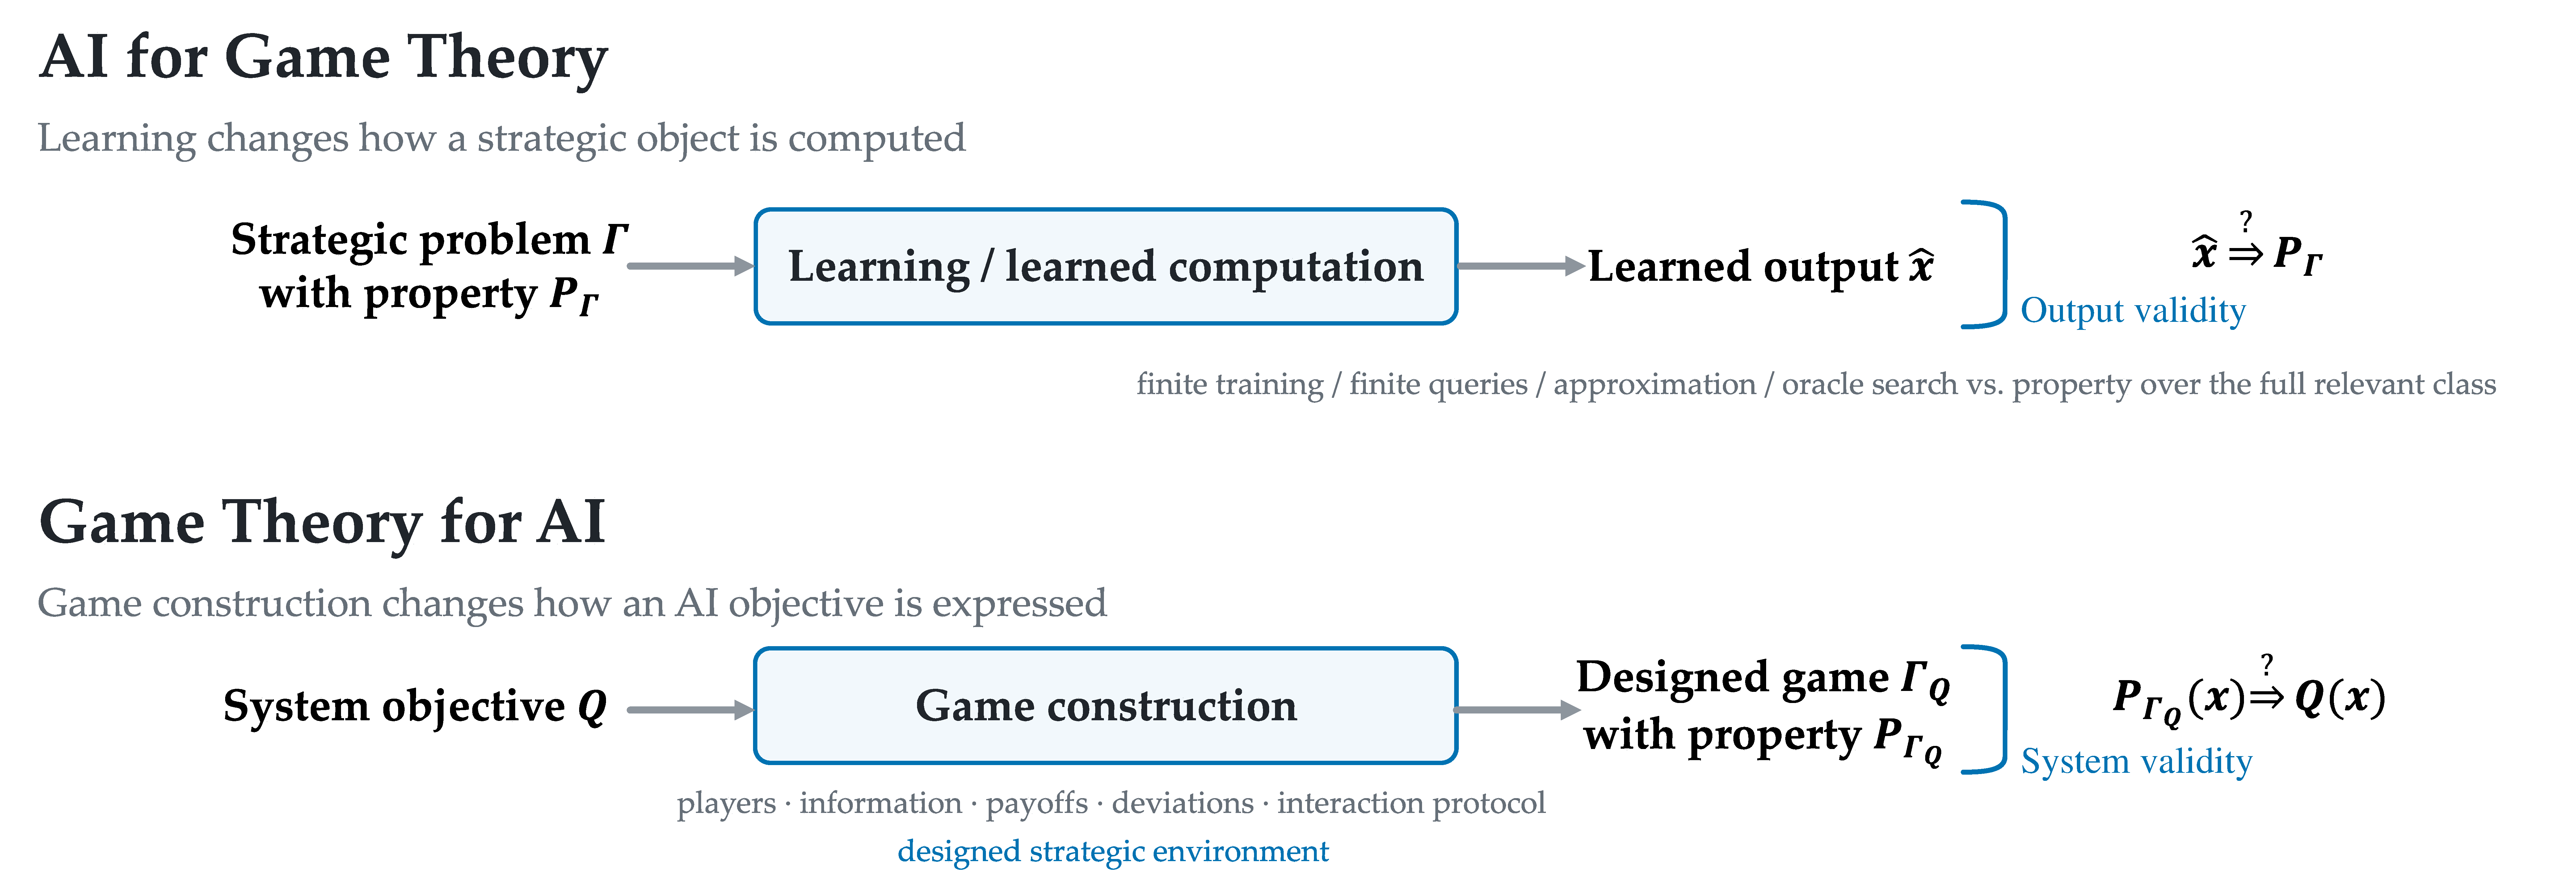
\includegraphics[width=\textwidth]{figure/fig1-preservation-gaps.pdf}
\caption{The two validity questions. \emph{Output validity} concerns the
strategic property of a learned output. \emph{System validity} concerns whether
a property established inside a designed game supports the game's external
objective. Section~\ref{sec:synthesis} gives the conditions for composing the
two implications.}
\label{fig:validity-gates}
\end{figure}

\subsection{Why the Distinction Matters}
\label{sec:intro:why}

The distinction matters when learned strategic systems are evaluated beyond a
fixed benchmark. Field evidence from retail gasoline markets links algorithmic
pricing to higher margins~\citep{Assad2024}. In oligopoly experiments,
language-model agents reach supra-competitive prices without
instruction~\citep{FishGonczarowskiShorrer2024}. Language models also propose
executable mechanisms and equilibrium derivations
~\citep{PrimeNash2025,LegoNE2025,LiuGuoConitzer2025}. These outputs can be
checked mechanically against a formal specification. Executability alone does
not supply that specification or establish the strategic claim.

The same evidentiary question appears in proposals to regulate algorithmic
collusion. These proposals ask whether a firm can produce evidence that its
pricing algorithm was not exploiting its rivals, with the burden of producing
that evidence assigned by
rule~\citep{HartlineLongZhang2024,HartlineWangZhang2025,Harrington2018}. When a
statistical property of a deployment log is offered as a legal defense, the
scope of the claim supported by that finite evidence becomes part of the
proposed regulatory design.

\subsection{Scope and How to Read This Survey}
\label{sec:intro:scope}

\paragraph{Scope.} We study systems that learn strategic rules from data or
interaction. A high-dimensional trained rule may require empirical queries
and statistical bounds, whereas executable code or membership in a structured
family may permit direct checking. The appropriate analysis therefore depends
on the representation and the property being claimed.

\paragraph{Related surveys and exclusions.} Stackelberg
and security games, mean-field games, multi-agent reinforcement learning beyond
its use as a response oracle, autobidding, and incentive design for federated
learning fall outside our selected domains. \citet{WellmanTuylsGreenwald2025}
and \citet{CurryAMDSurvey2025} provide focused reviews of empirical
game-theoretic analysis and automated mechanism design, respectively.
\citet{SunWuChengChu2025} survey the game theory--LLM intersection with the
language model as the focal technology. \citet{Podimata2025} surveys
incentive-aware machine learning, where individuals adapt their inputs to a
deployed decision rule. Each of these surveys organizes the literature around
its object of study. We organize by the relation between a computation, the claim attached
to it, and the evidence available for that claim.

\paragraph{Organization.} Section~\ref{sec:recap} introduces the computational
background. Sections~\ref{sec:ai4gt} and~\ref{sec:gt4ai} organize six application
areas around the two validity questions, as illustrated in
Figure~\ref{fig:survey-route}. Section~\ref{sec:synthesis} states when the two
can be combined. After deployment, participants' responses can alter the inputs
and counterparties that the system encounters. Performative prediction
provides one formalization of such feedback~\citep{Perdomo2020Performative}. A
guarantee established on a fixed evaluation distribution need not extend to the
deployment distribution shaped by those responses. The relevant response
process and case domain must therefore be specified as part of the claim.

\begin{figure}[pos=ht]
\centering
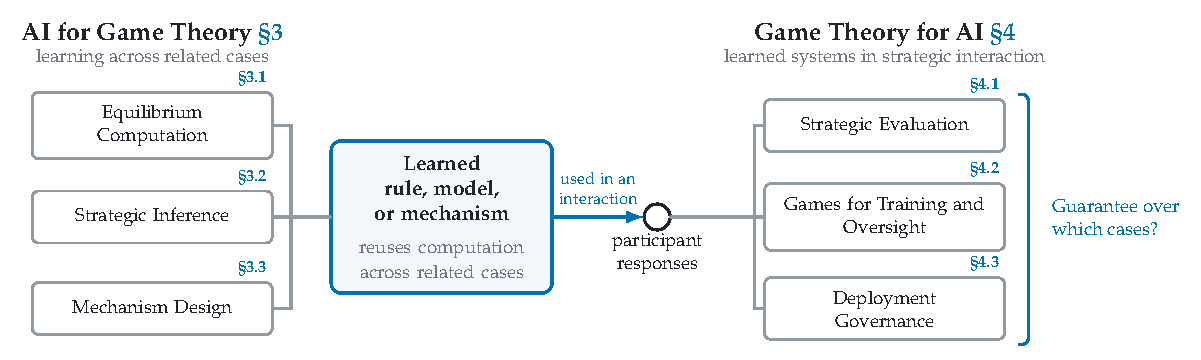
\includegraphics[width=0.9\textwidth]{figure/fig2-survey-route.pdf}
\caption{Survey structure and the interaction link. Section~3 studies learned
strategic objects across related cases. Section~4 studies learned systems in
interactions where participant responses can change the relevant cases. The
six labels identify the corresponding subsections and need not be disjoint.}
\label{fig:survey-route}
\end{figure}

\FloatBarrier
